\section{BLAST Results}\label{section:blast}

To determine if gene finders predict genes that are present in other similar species, proteins from three related organisms were used as
queries to tblastn\cite{altschul1990a} on each \textit{Trichoderma}
assembly. The organisms and their associated NCBI accession IDs are as
follows: \textit{T. atroviride} \- GCF\_000171015.1,
\textit{F. graminarium} \- GCF\_000240135.3, \textit{S. cerevisiae} \-
GCF\_000146045.2.  Results from the tblastn runs are presented in
Figure~\ref{fig:blast-total-counts} and Table~\ref{table:tblastn-prots}. Initial tblastn results appear
promising for both the \textit{T. atroviride} and \textit{Fusarium}
datasets. All assemblies considered contain at minimum 89\% of the
reference protein sequences in the case of \textit{T. atroviride} and
a minimum of 75\% in the case of \textit{Fusarium}. In the case of
\textit{S. cerevisiae}, a minimum of 57\% of reference proteins
matched. It appears that the percentage of hits decreases as
evolutionary distance increases. These results provide rough
validation that the assemblies contain potential for protein coding
sequences.

\begin{figure}
  \centering
  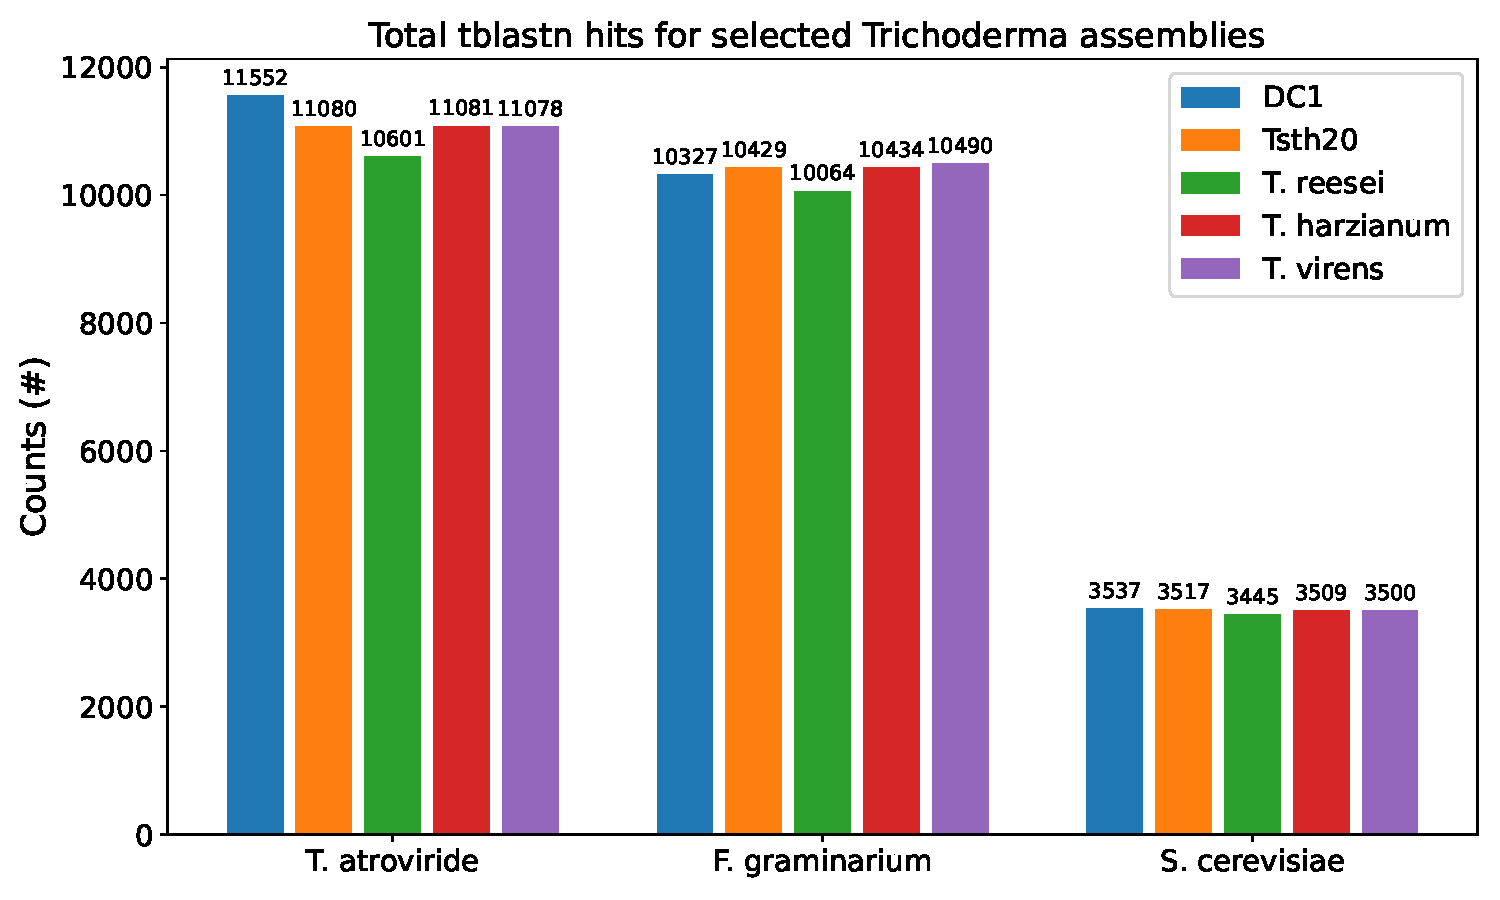
\includegraphics[width=0.85\textwidth]{figures/blast-total-counts.pdf}
  \caption[Total tblastn hits]{Total tblastn hits for reference proteins from \textit{T. atroviride}, \textit{F. graminarium}, and \textit{S. cerevisiae} against \textit{Trichoderma} assemblies.}\label{fig:blast-total-counts}
\end{figure}

\begin{table}
  \centering
  \begin{tabular}{|c|c|c|c|c|c|c|}
    \hline
    Reference & Ref. Proteins & DC1 & Tsth20 & \textit{T. reesei} & \textit{T. harzianum} & \textit{T. virens}  \\ \hline
    \textit{Trichoderma atroviride} & 11807 & 11552 & 11080 & 10601 & 11081 & 11078 \\ \hline 
    \textit{Fusarium graminarium} & 13312 & 10327 & 10429 & 10064 & 10434 & 10490 \\ \hline
    \textit{Saccharomyces cerevisiae} & 6014 & 3537 & 3517 & 3445 & 3509 & 3500 \\ \hline
  \end{tabular}
  \caption[Overview of tblastn alignments]{tblastn hits from reference protein sequences to selected
    \textit{Trichoderma} assemblies. Hits are reported if the
    alignment length is greater than 30\% of the reference protein
    length and if 30\% of the alignment length has identical
    matches.}\label{table:tblastn-prots}
\end{table}

While successful tblastn hits from input proteins are useful, it is
worthwhile exploring those hits in the context of regions and gene
predictions within them. Counts of genes from regions with tblastn
hits are shown in Figures~\ref{fig:blast-tatroviride},~\ref{fig:blast-fgraminarium},~\ref{fig:blast-scerevisiae}, and Table~\ref{table:tblastn-genes}. In a similar trend
to Table~\ref{table:tblastn-prots}, genes in regions with tblastn hits
decrease as evolutionary distance increases. In DC1 and Tsth20, we
observe that Braker2 predicts more genes in regions with tblastn hits
than GeneMark. RefSeq is not included for DC1 and Tsth20, as there is
no RefSeq annotation available. In \textit{T. harzianum} and
\textit{T. virens}, Braker2 and RefSeq appear to have similar counts
of genes in regions with tblastn hits. Interestingly, in the case of
\textit{T. reesei}, there are more genes from GeneMark in regions with
tblastn hits, which is not the case in \textit{T. harzianum} and
\textit{T. virens}.

Another interesting observation is comparing the coverage, or
completeness, of the input and query sequence. As mentioned, it
appears that high proportions of query sequences are being mapped to
the subject, but the gene predictions are not as well represented in
regions where those tblastn hits occur. A likely reason for this is
inappropriate alignment parameters. More flexible gap parameters and
the use of a different scoring matrix would likely produce better
results, but optimization of parameters was not performed in this
analysis. It is also possible that the post-alignment filtering
criteria were inappropriate, resulting in short alignments that are
true in nature, but may not be indicative of the presence of a truly
similar protein.

\begin{figure}[htp]
  \centering
  \begin{subfigure}[b]{0.85\textwidth}
    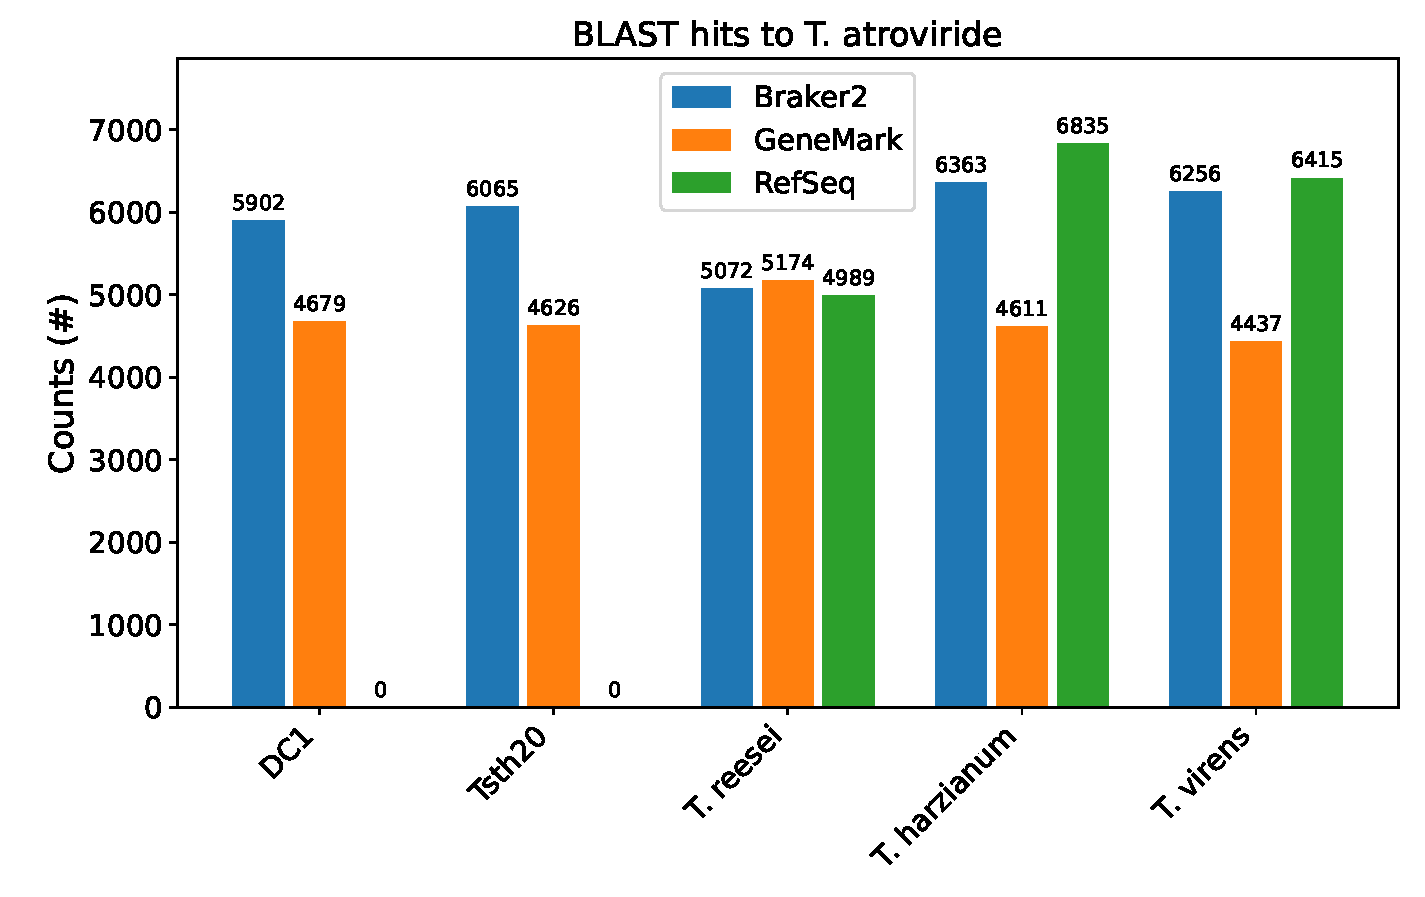
\includegraphics[width=\textwidth]{figures/blast-tatroviride.pdf}
    \caption{\textit{T. atroviride} tblastn hits}\label{fig:blast-tatroviride}
  \end{subfigure}
  \par\medskip
  \begin{subfigure}[b]{0.85\textwidth}
    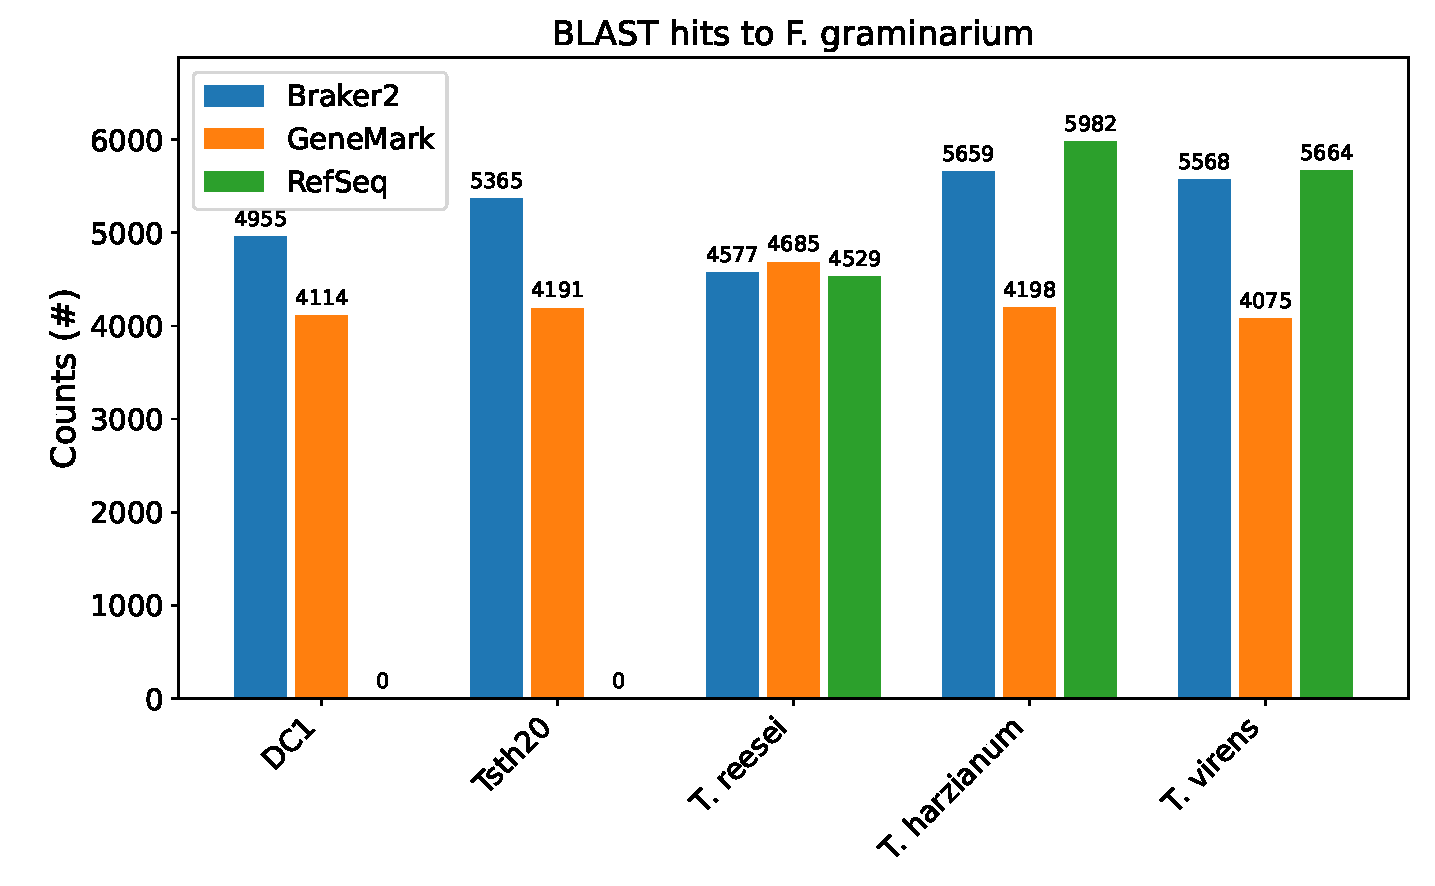
\includegraphics[width=\textwidth]{figures/blast-fgraminarium.pdf}
    \caption{\textit{F. graminarium} tblastn hits}\label{fig:blast-fgraminarium}
  \end{subfigure}
\end{figure}
\begin{figure}[htp]\ContinuedFloat
  \centering
  \begin{subfigure}[b]{0.85\textwidth}
    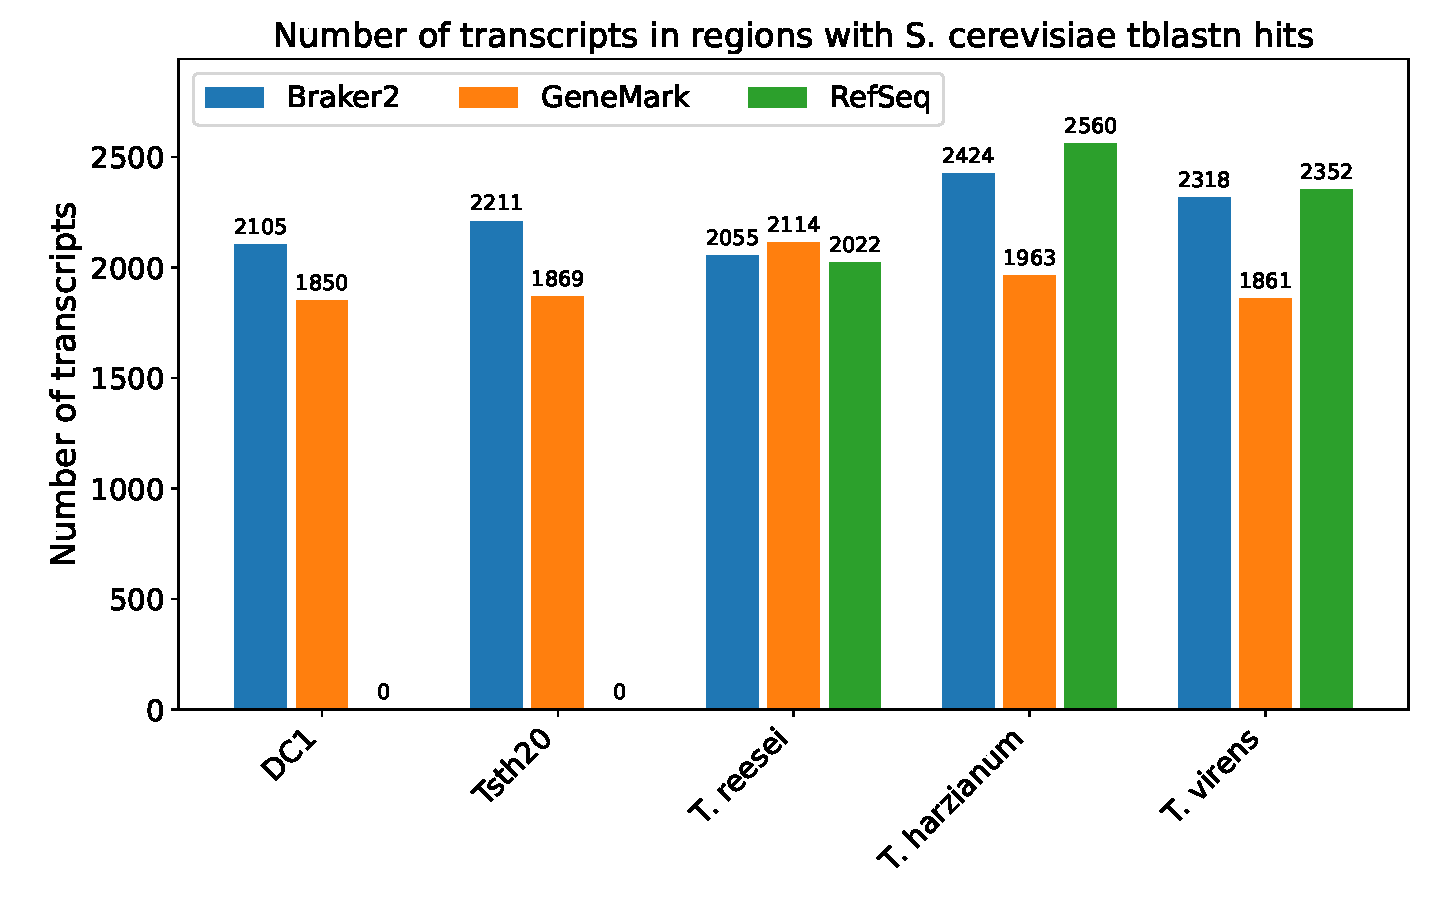
\includegraphics[width=\textwidth]{figures/blast-scerevisiae.pdf}
    \caption{\textit{S. cerevisiae} tblastn hits}\label{fig:blast-scerevisiae}
  \end{subfigure}
  \caption[Results from tblastn by reference]{tblastn hits for reference proteins from \textit{T. atroviride}, \textit{F. graminarium}, and \textit{S. cerevisiae} against \textit{Trichoderma} assemblies. For DC1 and Tsth20, RefSeq annotations are not available, so their values are set to 0.}\label{fig:blast-hits}
\end{figure}

\begin{table}
  \centering
  \begin{tabular}{|c|c|c|c|c|}
    \hline
    Subject & Query & Braker2 & GeneMark & RefSeq \\ \hline
    DC1 & \textit{T. atroviride} & 5902 & 4679 & N/A \\ \hline
    DC1 & \textit{F. graminarium} & 4955 & 4114 & N/A \\ \hline
    DC1 & \textit{S. cerevisiae} & 2105 & 1850 & N/A \\ \hline
    Tsth20 & \textit{T. atroviride} & 6065 & 4626 & N/A \\ \hline
    Tsth20 & \textit{F. graminarium} & 5365 & 4191 & N/A \\ \hline
    Tsth20 & \textit{S. cerevisiae} & 2211 & 1869 & N/A \\ \hline
    \textit{T. reesei} & \textit{T. atroviride} & 5072 & 5174 & 4989 \\ \hline
    \textit{T. reesei} & \textit{F. graminarium} & 4577 & 4685 & 4529 \\ \hline
    \textit{T. reesei} & \textit{S. cerevisiae} & 2055 & 2114 & 2022 \\ \hline
    \textit{T. harzianum} & \textit{T. atroviride} & 6363 & 4611 & 6835 \\ \hline
    \textit{T. harzianum} & \textit{F. graminarium} & 5659 & 4198 & 5982 \\ \hline
    \textit{T. harzianum} & \textit{S. cerevisiae} & 2424 & 1963 & 2560 \\ \hline
    \textit{T. virens} & \textit{T. atroviride} & 6256 & 4437 & 6415 \\ \hline
    \textit{T. virens} & \textit{F. graminarium} & 5568 & 4075 & 5664 \\ \hline
    \textit{T. virens} & \textit{S. cerevisiae} & 2318 & 1861 & 2352 \\ \hline
  \end{tabular}
  \caption[Counts of transcripts in regions with tblastn hits]{Counts of transcripts predicted by Braker2, GeneMark and
    RefSeq in regions containing tblastn hits from
    \textit{Trichoderma atroviride}, \textit{Fusarium graminarium},
    and \textit{Saccharomyces cerevisiae}.}\label{table:tblastn-genes}
\end{table}

Overall, it appears that using tblastn with proteins from related
organisms may be a viable option as a control when no reference or
model organism is available. At the very minimum, tblastn hits can be
used as another piece of supporting evidence for the existence of a
gene, with one caveat being imperfect coverage of predictions. The
issue of imperfect coverage may be mitigated by parameter
optimization. It is also possible that one could employ a
similarity-based cutoff on the proportion of predicted genes in
regions with tblastn hits as an indicator of gene finding performance;
however, this would require further analysis, preferably with more
closely related organisms.
